
Let us start with ${\cal A}_e$ where we assume that $k$ is constant within an element:
\begin{eqnarray}
{\cal A}_{\Omega_e}&=&
\left(
\begin{array}{ccc}
\int_\Omega \vec{N}^T \vec{N} dV & 0 & -\int_\Omega k \partial_x \vec{N}^T \vec{N} \; dV \\ \\
0 & \int_\Omega \vec{N}^T \vec{N} dV & -\int_\Omega k \partial_y \vec{N}^T \vec{N} \; dV \\ \\
- \int_{\Omega} \partial_x \vec{N}^T \vec{N}   \; dV & 
- \int_{\Omega} \partial_y \vec{N}^T \vec{N}   \; dV & 0 
\end{array}
\right) \\
&=&
\left(
\begin{array}{ccc}
0 & - \int_{\Omega} \partial_x \vec{N}^T \vec{N}   \; dV  & - \int_{\Omega} \partial_y \vec{N}^T \vec{N}   \; dV  \\ \\
-k_e \int_\Omega \partial_x \vec{N}^T \vec{N} \; dV & \int_\Omega \vec{N}^T\vec{N} dV & 0 \\  \\
-k_e \int_\Omega \partial_y \vec{N}^T \vec{N} \; dV & 0 & \int_\Omega \vec{N}^T\vec{N} dV  
\end{array}
\right) \nn\\
&=&
\left(
\begin{array}{ccc}
0 & -{\bm J}_x & -{\bm J}_y \\
-{\bm H}_x & {\bm E} & 0 \\
-{\bm H}_y & 0 & {\bm E} 
\end{array}
\right) \nn\\
&=&
\left(
\begin{array}{ccc}
0 & -{\bm J}_x & -{\bm J}_y \\
-k_e{\bm J}_x & {\bm E} & 0 \\
-k_e{\bm J}_y & 0 & {\bm E} 
\end{array}
\right)
\end{eqnarray}

For $Q_1$ shape functions the vector $\vec{N}$ is $(N_1(r,s),N_2(r,s),N_3(r,s),N_4(r,s))$ and under the assumption 
that elements are rectangles of size $h_x$ and $h_y$ we obtain. 
\begin{eqnarray}
{\bm E} 
&=&\int_\Omega \vec{N}^T \vec{N} dV  \nn\\
&=& \int_{\Omega_e} \vec{N}^T(x,y) \vec{N}(x,y)\;  dx dy  \nn\\
&=& \frac{h_xh_y}{4} \int_{-1}^{+1} \int_{-1}^{+1} \vec{N}^T(r,s) \vec{N}(r,s)\;  dr ds  \nn\\
&=& \frac{h_x h_y}{9}\left(
\begin{array}{cccc}
1 & \frac{1}{2} & \frac{1}{4} & \frac{1}{2}\\
\frac{1}{2}&  1& \frac{1}{2} & \frac{1}{4}\\ 
\frac{1}{4} & \frac{1}{2} & 1 & \frac{1}{2}\\
\frac{1}{2} & \frac{1}{4} & \frac{1}{2} & 1
\end{array}
\right) 
\nn\\
{\bm J}_x &=& \int_\Omega \partial_x\vec{N}^T \vec{N} dV  \nn\\
&=& \int_{\Omega_e} \partial_x\vec{N}^T(x,y) \vec{N}(x,y)\;  dx dy  \nn\\
&=& \frac{h_xh_y}{4} \int_{-1}^{+1} \int_{-1}^{+1} \partial_r\vec{N}^T(r,s) \vec{N}(r,s)\;  dr ds  \nn\\
&=& \frac{h_y}{12}
\left(\begin{array}{cccc}
-2 & 2 & 1 & -1\\
-2 & 2  &  1 & -1\\
-1 & 1  &  2 & -2\\
-1 & 1 & 2 &-2
\end{array}
\right)
\nn\\
{\bm J}_y &=&
\int_\Omega \partial_y\vec{N}^T \vec{N} dV \nn\\
&=& \int_{\Omega_e} \partial_y\vec{N}^T(x,y) \vec{N}(x,y)\;  dx dy  \nn\\
&=& \frac{h_xh_y}{4} \int_{-1}^{+1} \int_{-1}^{+1} \partial_s\vec{N}^T(r,s) \vec{N}(r,s)\;  dr ds \nn \\
&=&\frac{h_x}{12}
\left(\begin{array}{cccc}
-2 & -1 & 1 & 2\\
-1 & -2 & 2 & 1\\
-1 & -2 & 2 & 1\\
-2 & -1 & 1 & 2
\end{array}
\right) \nn
\end{eqnarray}
\todo[inline]{verify M, Jx, Jy expressions?}

The matrix ${\cal A}_{\Omega_e}$ is therefore trivial to implement. 



\newpage
Let us now turn to $ {\cal A}_{\partial\Omega}$ which is specific to the DG method.
Because elements are rectangles then $n_i^+n_j^+=0$ if $i \neq j$. 
Also, if $i=j$ then $n_i^+n_j^+=1$. 


\begin{center}
\includegraphics[width=7cm]{images/dgfem/dgelts_q1}
\end{center}

Assuming here again that heat conductivities are constant inside an element
it then follows that 
\begin{eqnarray}
 {\cal A}_{\partial\Omega_e}
&=&
\left(
\begin{array}{ccc}
-  {\cal{E}} \int_{\partial\Omega}     \vec{N}^T \vec{N} dS   & 
\int_{\partial\Omega}  \left(\frac{1}{2} - \vec{\cal{C}} \cdot \vec{n}^+ \right) \vec{N}^T \vec{N} n^+_x  \; dS &
  \int_{\partial\Omega}  \left(\frac{1}{2} - \vec{\cal{C}} \cdot \vec{n}^+ \right) \vec{N}^T \vec{N} n^+_y  \; dS \\ \\
k_e \int_{\partial\Omega}  \left( \frac{1}{2} + \vec{\cal C} \cdot \vec{n}^+ \right) {N}^T \vec{N} n^+_x dS & 
-k_e\int_{\partial\Omega}  \vec{N}^T\vec{N}  {\cal F} {n}^+_x   n^+_x dS  
& 0 \\ \\
k_e \int_{\partial\Omega}  \left( \frac{1}{2} + \vec{\cal C} \cdot \vec{n}^+ \right) {N}^T \vec{N} n^+_y dS & 
0
& -k_e \int_{\partial\Omega}  \vec{N}^T\vec{N}  {\cal F} {n}^+_y   n^+_y dS    
\end{array}
\right)
\nn\\
&=&
\sum_{i=1}^{nedges}
\left(
\begin{array}{ccc}
-  {\cal{E}} \int_{\partial\Omega_i}     \vec{N}^T \vec{N} dS   & 
\int_{\partial\Omega_i}  \left(\frac{1}{2} - \vec{\cal{C}} \cdot \vec{n}^+ \right) \vec{N}^T \vec{N} n^+_x  \; dS &
  \int_{\partial\Omega_i}  \left(\frac{1}{2} - \vec{\cal{C}} \cdot \vec{n}^+ \right) \vec{N}^T \vec{N} n^+_y  \; dS \\ \\
k_e \int_{\partial\Omega_i}  \left( \frac{1}{2} + \vec{\cal C} \cdot \vec{n}^+ \right) {N}^T \vec{N} n^+_x dS & 
-k_e\int_{\partial\Omega_i}  \vec{N}^T\vec{N}  {\cal F} {n}^+_x   n^+_x dS  
& 0 \\ \\
k_e \int_{\partial\Omega_i}  \left( \frac{1}{2} + \vec{\cal C} \cdot \vec{n}^+ \right) {N}^T \vec{N} n^+_y dS & 
0
& -k_e \int_{\partial\Omega_i}  \vec{N}^T\vec{N}  {\cal F} {n}^+_y   n^+_y dS    
\end{array}
\right) \nn\\
&=&
\sum_{i=1}^{nedges}
\left(
\begin{array}{ccc}
{\bm G}_i & {\bm J}_{x,i} & {\bm J}_{y,i} \\
{\bm H}_{x,i} & {\bm E}_{xx,i} & 0 \\ 
{\bm H}_{y,i} & 0 & {\bm E}_{yy,i} 
\end{array}
\right) \nn
\end{eqnarray}

Note that 
\begin{itemize}
\item $i=1$: bottom edge, i.e. $s=-1$ and then $N_4=N_3=0$,
\item $i=2$: right  edge, i.e.  $r=+1$ and then $N_1=N_4=0$,
\item $i=3$: top edge, i.e. $s=+1$  and then $N_1=N_2=0$,
\item $i=4$: left edge, i.e. $r=-1$ and then $N_2=N_3=0$.
\end{itemize}


\begin{eqnarray}
{\bm G}_1 &=& -  {\cal{E}} \int_{\partial\Omega_1} \vec{N}^T \vec{N} dS = -  {\cal{E}} {\bm C}_1 \nn\\
{\bm G}_2 &=& -  {\cal{E}} \int_{\partial\Omega_2} \vec{N}^T \vec{N} dS = -  {\cal{E}} {\bm C}_2 \nn\\
{\bm G}_3 &=& -  {\cal{E}} \int_{\partial\Omega_3} \vec{N}^T \vec{N} dS = -  {\cal{E}} {\bm C}_3 \nn\\
{\bm G}_4 &=& -  {\cal{E}} \int_{\partial\Omega_4} \vec{N}^T \vec{N} dS = -  {\cal{E}} {\bm C}_4 \nn\\
\end{eqnarray}
with 
\begin{eqnarray}
{\bm C}_{1} 
&=& \int_{1\rightarrow 2} \vec{N}^T \vec{N} dS  \nn\\
&=& 
\frac{h_x}{2}
\int_{-1}^{+1}  
\left(\begin{array}{cccc}
N_1(r,-1)N_1(r,-1) & N_1(r,-1) N_2(r,-1) & 0 & 0 \\
N_2(r,-1)N_1(r,-1) & N_2(r,-1) N_2(r,-1) & 0 & 0 \\
0 & 0 & 0 & 0 \\
0 & 0 & 0 & 0 
\end{array}\right)
ds \nn\\
&=&
\frac{h_x}{6}
\left(\begin{array}{cccc}
2 & 1 & 0 & 0 \\
1 & 2 & 0 & 0 \\
0 & 0 & 0 & 0 \\
0 & 0 & 0 & 0 
\end{array}\right)
\nn\\
\nn\\
{\bm C}_{2} 
&=& \int_{2\rightarrow 3} \vec{N}^T \vec{N} dS  \nn\\
&=& 
\frac{h_y}{2}
\int_{-1}^{+1}  
\left(\begin{array}{cccc}
0 & 0 & 0 & 0 \\
0 & N_2(+1,s)N_2(+1,s) & N_2(+1,s) N_3(+1,s) &0\\
0 & N_3(+1,s)N_2(+1,s) & N_3(+1,s) N_3(+1,s) &0\\
0 & 0 & 0 & 0 
\end{array}\right)
ds 
\nn\\
&=&
\frac{h_y}{6}
\left(\begin{array}{cccc}
0 & 0 & 0 & 0 \\
0 & 2 & 1 & 0 \\
0 & 1 & 2 & 0 \\
0 & 0 & 0 & 0 
\end{array}\right)
\nn\\
{\bm C}_{3}
&=& \int_{3\rightarrow 4} \vec{N}^T \vec{N} dS \nn\\
&=& -\int_{4\rightarrow 3} \vec{N}^T \vec{N} dS \nn\\
&=& 
-\frac{h_x}{2}
\int_{-1}^{+1}  
\left(\begin{array}{cccc}
0 & 0 & 0 & 0 \\
0 & 0 & 0 & 0 \\ 
0 & 0 & N_3(r,+1)N_3(r,+1) & N_3(r,+1) N_4(r,+1) \\
0 & 0 & N_4(r,+1)N_3(r,+1) & N_4(r,+1) N_4(r,+1)
\end{array}\right)
ds \nn\\
&=&
-\frac{h_x}{6}
\left(\begin{array}{cccc}
0 & 0 & 0 & 0 \\
0 & 0 & 0 & 0 \\
0 & 0 & 2 & 1 \\
0 & 0 & 1 & 2 
\end{array}\right)
\nn\\
\nn\\
{\bm C}_{4} 
&=& \int_{4\rightarrow 1} \vec{N}^T \vec{N} dS  \nn\\
&=& -\int_{1\rightarrow 4} \vec{N}^T \vec{N} dS  \nn\\
&=& 
-\frac{h_y}{2}
\int_{-1}^{+1}  
\left(\begin{array}{cccc}
N_1(-1,s)N_1(-1,s) & 0 & 0 & N_1(-1,s) N_4(-1,s) \\
0 & 0 & 0 & 0 \\
0 & 0 & 0 & 0 \\
N_1(-1,s)N_4(-1,s) & 0 & 0 & N_4(-1,s) N_4(-1,s)
\end{array}\right)
ds \nn\\
&=& 
-\frac{h_y}{2}
\int_{-1}^{+1}  
\left(\begin{array}{cccc}
(1-s)^2/4 &0 & 0 & (1-s^2)/4 \\
0 & 0 & 0 & 0 \\
0 & 0 & 0 & 0 \\
(1-s^2)/4 & 0 & 0 & (1+s)^2/4 
\end{array}\right)
ds \nn\\
&=&
-\frac{h_y}{8}
\left(\begin{array}{cccc}
8/3 & 0 & 0 & 4/3 \\
0 & 0 & 0 & 0 \\
0 & 0 & 0 & 0 \\
4/3& 0 & 0 & 8/3 
\end{array}\right)
\nn\\
&=&
-\frac{h_y}{6}
\left(\begin{array}{cccc}
2 & 0 & 0 & 1 \\
0 & 0 & 0 & 0 \\
0 & 0 & 0 & 0 \\
1& 0 & 0 & 2 
\end{array}\right)
\nn
\end{eqnarray}

\begin{eqnarray}
{\bm E}_{xx,1} &=& -k_e {\cal F} \int_{\partial\Omega_1}  \vec{N}^T\vec{N}  {n}^+_x   n^+_x dS = 0 \nn\\ 
{\bm E}_{xx,2} &=& -k_e {\cal F} \int_{\partial\Omega_2}  \vec{N}^T\vec{N}  {n}^+_x   n^+_x dS = -k_e {\cal F} {\bm C}_2  \nn\\ 
{\bm E}_{xx,3} &=& -k_e {\cal F} \int_{\partial\Omega_3}  \vec{N}^T\vec{N}  {n}^+_x   n^+_x dS = 0 \nn\\ 
{\bm E}_{xx,4} &=& -k_e {\cal F} \int_{\partial\Omega_4}  \vec{N}^T\vec{N}  {n}^+_x   n^+_x dS = -k_e {\cal F} {\bm C}_4  
\nn\\
{\bm E}_{yy,1} &=& -k_e {\cal F} \int_{\partial\Omega_1}  \vec{N}^T\vec{N}  {n}^+_y   n^+_y dS = -k_e {\cal F} {\bm C}_1  \nn\\ 
{\bm E}_{yy,2} &=& -k_e {\cal F} \int_{\partial\Omega_2}  \vec{N}^T\vec{N}  {n}^+_y   n^+_y dS = 0 \nn\\ 
{\bm E}_{yy,3} &=& -k_e {\cal F} \int_{\partial\Omega_3}  \vec{N}^T\vec{N}  {n}^+_y   n^+_y dS = -k_e {\cal F} {\bm C}_3  \nn\\  
{\bm E}_{yy,4} &=& -k_e {\cal F} \int_{\partial\Omega_4}  \vec{N}^T\vec{N}  {n}^+_y   n^+_y dS = 0 
\nn\\ 
{\bm H}_{x,1} &=& k_e \int_{\partial\Omega_1}  \left( \frac{1}{2} + \vec{\cal C} \cdot \vec{n}^+ \right) \vec{N}^T \vec{N} n^+_x dS = 0 \nn\\ 
{\bm H}_{x,2} &=& k_e \int_{\partial\Omega_2}  \left( \frac{1}{2} + \vec{\cal C} \cdot \vec{n}^+ \right) \vec{N}^T \vec{N} n^+_x dS = k_e  \left( \frac{1}{2} + {\cal C}_x \right) {\bm C}_{2} \nn\\ 
{\bm H}_{x,3} &=& k_e \int_{\partial\Omega_3}  \left( \frac{1}{2} + \vec{\cal C} \cdot \vec{n}^+ \right) \vec{N}^T \vec{N} n^+_x dS = 0 \nn\\ 
{\bm H}_{x,4} &=& k_e \int_{\partial\Omega_4}  \left( \frac{1}{2} + \vec{\cal C} \cdot \vec{n}^+ \right) \vec{N}^T \vec{N} n^+_x dS = - k_e  \left( \frac{1}{2} - {\cal C}_x \right) {\bm C}_{4} 
\nn\\
{\bm H}_{y,1} &=& k_e \int_{\partial\Omega_1}  \left( \frac{1}{2} + \vec{\cal C} \cdot \vec{n}^+ \right) \vec{N}^T \vec{N} n^+_y dS = -k_e  \left( \frac{1}{2} - {\cal C}_y \right) {\bm C}_{1} \nn\\ 
{\bm H}_{y,2} &=& k_e \int_{\partial\Omega_2}  \left( \frac{1}{2} + \vec{\cal C} \cdot \vec{n}^+ \right) \vec{N}^T \vec{N} n^+_y dS = 0 \nn\\ 
{\bm H}_{y,3} &=& k_e \int_{\partial\Omega_3}  \left( \frac{1}{2} + \vec{\cal C} \cdot \vec{n}^+ \right) \vec{N}^T \vec{N} n^+_y dS = k_e  \left( \frac{1}{2} + {\cal C}_y \right) {\bm C}_{3} \nn\\ 
{\bm H}_{y,4} &=& k_e \int_{\partial\Omega_4}  \left( \frac{1}{2} + \vec{\cal C} \cdot \vec{n}^+ \right) \vec{N}^T \vec{N} n^+_y dS = 0 \nn\\ 
\nn\\
{\bm J}_{x,1} &=& \int_{\partial\Omega_1}  \left(\frac{1}{2} - \vec{\cal{C}} \cdot \vec{n}^+ \right) \vec{N}^T \vec{N} n^+_x  \; dS = 0 \nn\\ 
{\bm J}_{x,2} &=& \int_{\partial\Omega_2}  \left(\frac{1}{2} - \vec{\cal{C}} \cdot \vec{n}^+ \right) \vec{N}^T \vec{N} n^+_x  \; dS = \left(\frac{1}{2} - {\cal C}_x \right) {\bm C}_{2} \nn\\
{\bm J}_{x,3} &=& \int_{\partial\Omega_3}  \left(\frac{1}{2} - \vec{\cal{C}} \cdot \vec{n}^+ \right) \vec{N}^T \vec{N} n^+_x  \; dS = 0 \nn\\
{\bm J}_{x,4} &=& \int_{\partial\Omega_4}  \left(\frac{1}{2} - \vec{\cal{C}} \cdot \vec{n}^+ \right) \vec{N}^T \vec{N} n^+_x  \; dS = -\left(\frac{1}{2} + {\cal C}_x \right) {\bm C}_{4} \nn\\
\nn\\
{\bm J}_{y,1} &=& \int_{\partial\Omega_1}  \left(\frac{1}{2} - \vec{\cal{C}} \cdot \vec{n}^+ \right) \vec{N}^T \vec{N} n^+_y  \; dS = - \left(\frac{1}{2} + {\cal C}_y \right) {\bm C}_{1} \nn\\
{\bm J}_{y,2} &=& \int_{\partial\Omega_2}  \left(\frac{1}{2} - \vec{\cal{C}} \cdot \vec{n}^+ \right) \vec{N}^T \vec{N} n^+_y  \; dS = 0 \nn\\
{\bm J}_{y,3} &=& \int_{\partial\Omega_3}  \left(\frac{1}{2} - \vec{\cal{C}} \cdot \vec{n}^+ \right) \vec{N}^T \vec{N} n^+_y  \; dS =   \left(\frac{1}{2} - {\cal C}_y \right) {\bm C}_{3} \nn\\
{\bm J}_{y,4} &=& \int_{\partial\Omega_4}  \left(\frac{1}{2} - \vec{\cal{C}} \cdot \vec{n}^+ \right) \vec{N}^T \vec{N} n^+_y  \; dS = 0 \nn
\end{eqnarray}













